\chapter{Justificaci\'on}
\label{chp:just}

La locomoci\'on de las especies y el comportamiento de las mismas est\'an fuertemente relacionados. Su evoluci\'on y desarrollo est\'an guiados por su necesidad de adaptaci\'on al entorno. La adaptaci\'on es guiada principalmente por prueba-y-error a todo momento. La naturaleza del entorno por su complejidad hace que un individuo no tenga pleno conocimiento de su entorno y ante ello sus comportamientos deben ser robustos ante eventos imprevistos del entorno y su propio cuerpo.

La forma en que un individuo percibe su entorno se encuentra llena de perturbaciones y ruidos, que no le permiten tener total certeza del estado de s\'i mismo y del entorno. Sin embargo con esa informaci\'on incompleta y ruidosa, ese ser vivo debe tomar decisiones que lo mantengan internamente satisfecho. Los seres vivos no solo toman decisiones de lo que perciben en un instante, para ellos las percepciones inmediatamente pasadas y las experiencias de acciones o secuencia de acciones tomadas en situaciones anteriores son de suma importancia.

El individuo o agente vivo debe ser capaz no solo de percibir, sino tambien de tomar esa percepci\'on sensorial y convertirla o asociarla con un estado que represente la situaci\'on del mundo y de si mismo. Debido a esto el agente requiere de algo m\'as que no lo deje solo actuando de forma impulsiva y reflexiva sin pensar en sus consecuencias. El agente debe formar sus propios modelos de como se comporta el mundo con \'el mismo adentro y que efecto tienen sus aciones en su alrededor.

As\'i como sus percepciones no son certeras sus modelos tampoco lo ser\'an, pero tendr\'an un grado o porcentaje de acierto. Los modelos del mundo le servir\'an para hacer prediciones de acciones hipot\'eticas y con base en los estados hipot\'eticos obtenidos por dichas acciones, el agente podr\'a tomar la decisi\'on que m\'as le convenga. La conveniencia esta ligada a un objetivo. La representaci\'on y entendimiento interno del agente de dicho objetivo permite plantear en el individuo un mecanismo de aprendizaje y su tipo de aprendizaje.

\begin{figure}[!htb]
  \centering
  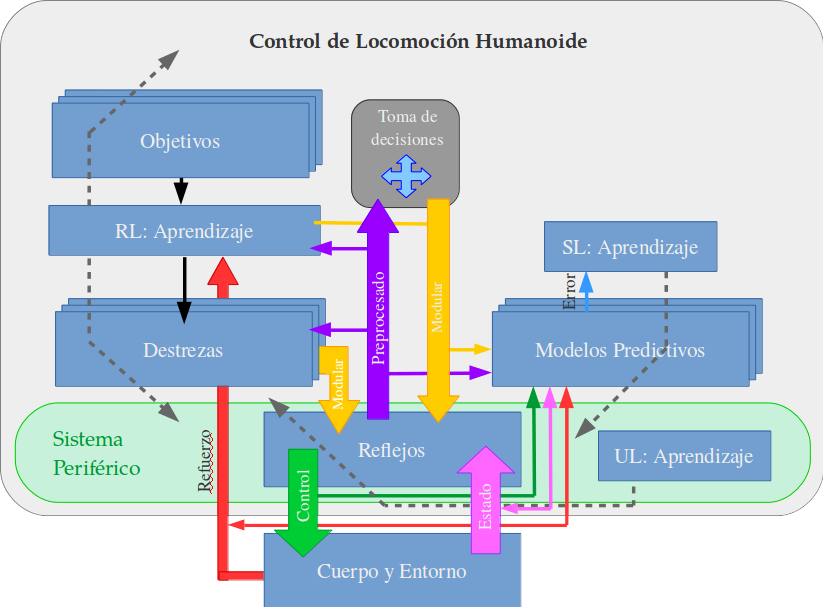
\includegraphics[width=1.0\textwidth]{images/ObjetivoGeneral.png}
  \caption{Estructura general de emergencia y aprendizaje de locomoci\'on basada en cognici\'on y reflejos}
  \label{fig:ObjGen}
\end{figure}

Importante: Resaltar el aporte del objetivo general en la ciencia.

% Ademas de utilizar hipotesis de las neurociencias y la psicolog\'ia, la rob\'otica ahora es utilizada para pruebas de hipotesis propuestas por estas dos ciencias, dando por creado la neuro-rob\'otica.

% Limitaciones
% \begin{itemize}
% \item Generaci\'on de trajectorias: por seguimiento[Citas], CPG[Citas] o HZD[Citas], se requiere que la estructura mec\'anica tienda a moverse sobre ciclos l\'imites. Sistemas autonomos y no-autonomos implicaciones de sincronizaci\'on.
% \item Basados en ZMP son quasi-est\'aticos[Citas]
% \item Limitaci\'on de los actuadores[Citas]
% \item Limitacion del sistema sensorial[Citas]
% \item Robustez a perturbaciones y habilidades ganadas.
% \item Adaptaci\'on de nuevos movimientos ante cambios del entorno y su necesidad a desempe\~narse
% \item Energ\'eticamente ineficientes
% \end{itemize}

% \par En la generaci\'on de trayectorias el empleo de redes bio-inspiradas de algunos insectos y animales son implementadas a trav\'es de los Central Pattern Generators presentes en el Sistema Nervioso Central \cite{Ijspeert2008}. Estas CPGs que representan osciladores acoplados (ver Figura \ref{fig:cpg}.) suelen configurar sus par\'ametros mediante algoritmos de optimizaci\'on, un ejemplo se puede ver en \cite{Kim2009} en el cual se usa enjambre de part\'iculas o por medio de aprendizeje Hebbiano \cite{Righetti2006a} este aprendizaje es guiado por lo general por una capa de control superior, denominada algunas veces Mesencephalic Locomotion Region {\textbf(MLR)}\cite{Shahbazi2012}.\\
% \par Otro caso que toma encuenta la interacci\'on de los sensores y los actuardores (ver Figura \ref{fig:SensingThroughBody}) para la formaci\'on de los reflejos, es una capa por lo general auto-organizada y presenta un aprendizaje no supervisado \cite{Iida2006,Manoonpong2007}. Posterior a estos trabajos \cite{Marques2013}, demuestra cuatro hip\'otesis de como se forman los reflejos apartir de la actividad espont\'anea de los actuadores o m\'usculos del agente y luego de su formaci\'on es posible la emergencia de un comportamiento coordinado, finalmente esta configuraci\'on permite adaptar su control a deficiencias morfol\'ogicas. En este \'ultimo trabajo se hace evidente el uso de aprendizaje supervisado y no supervisado.\\
% \par Por otra parte el aprendizaje por refuerzo ha sido utilizado para dise\~nar controles basados en control \'optimo y control adaptativo\cite{Wang2012a}. Las metodolog\'ias de Q-Learning y Actor-Critic han sido utilizadas con resultados notorios \cite{Tedrake2004}, en el que un agente logra la marcha en veinte minutos de aprendizaje. Q-learning es utilizado para el robot de la figura \ref{fig:SensingThroughBody} en \cite{Iida2009a}\\

% Control Robusto e inteligencia artificial

% Posibles reflejos: 
% Control tobillo, torso postura y posicionamiento del pie.
% ZMP, CoM, CoP, FRI, tiempo de duracion de la fase y longitud de paso. Velocidad promedio.


% Deep Learning. Aprendizaje por refuerzo.

% Como implementar?

% Robustez, versatilidad y eficiencia energ\'etica
% Sobre robustez: redundancia por medio de multiestrategias, usando el control de torque en el tobillo, la postura del torso  y el posicionamiento del pie.  Redundancia en la representacion reflexiva mediante la implementaci\'on morf\'ologica.

% Sobre versatilidad: La capacidad de adaptaci\'on. Aprendizaje y en especial la capacidad auto-organizaci\'on. La representaci\'on de conceptos o principios del la locomoci\'on b\'ipeda mediante Deep Learning.

% Sobre la eficiencia-energetica: El proceso de optimizacion, ya sea mediante algoritmos evolutivos o en general bio-inspirados, buscando hasta donde, con las restricciones tecnologicas nos permiten lograr un agente bipedo inteligente. Para esto la co-evoluci\'on de las estructuras de control y morfol\'ogicas deben ser dise\~nadas al tiempo

% Evaci\'on de obst\'aculos (bajo nivel) y navegacion (alto nivel- representaci\'on espacio-tiempo modelado) como ejercicios de planeaci\'on. Reflexivo e intencional \cite{Madani2011}.

% Observadores morfol\'ogicos, propiocepci\'on

% Control modular por niveles (reflexiva, memoria de destrezas, predictiva, creativa por motivacion, decisiva).
% Estructura b\'ipeda (basada en el modelo de \cite{Song2015}).
% Comportamiento racional (maximizando su recompenza futura, "tratar de hacer las cosas correctas").
% Reflejos auto-organizados ().
% Caracter\'isticas cognitivas (aprender, adaptarse, predecir y recordar).
% Computacion morfol\'ogica (forma de la implementaci\'on mediante la estructura mecanica o neuronal).
% Emergencia de locomoci\'on robusta y vers\'atil (programacion automatica).

% Exsiten desde el punto de la locomoci\'on b\'ipeda miles de esfuerzos por generar robots humanoides y no humanoides que sean capaces de caminar[Citas] o correr[Citas]. Adem\'as de estos esfuerzos por generar estructuras mec\'anicas que puedan moverse e interactuar como los humanos, existen n\'umerosos esfuerzos que intentan comprender la biomec\'anica del cuerpo humano probando hipotesis de forma computacional[Citas].

% ASIMO, HRP4 y NAO, son robots basados inicialmente en el concepto del ZMP, que es un movimiento ineficiente, con muy baja robustez aunque es versatil.
% Caminata din\'amica pasiva
% RABBIT, MABEL y MARLO capaces de correr y caminar
% PETMAN

% Desde el punto de vista biomec\'anico, el entendimiento del control de dicho sistema ha incluido la necesidad de entender y estudiar el sistema nervioso, y ante esto las teorias coneccionistas que incluyen las neurociencias han entrado a aportar difrentes hipotesis para el entendimiento de la locomoci\'on humanoide. Al estudiar el sistema neuronal nervioso, numerosas hipotesis y definiciones de conceptos aparecen. Las caracteristicas cognitivas deben son modeladas por diferentes redes neuronales.

% \par Generalmente la caminata b\'ipeda se analiza partiendo de muchos supuestos, un supuesto com\'un es anclar el pie soporte durate la fase de soporte simple. Como se demostr\'o en el trabajo de \cite{Chevallereau2008}, la fase de soporte doble es resumida en una din\'amica instant\'anea discreta que suele ser obviada ya que solo es necesaria su energ\'ia cin\'etica antes del impacto. Por esto en la mayoria de los analisis de marcha la fase de soporte doble es omitida y al asumir simetr\'ia en la marcha, el analisis queda reducido a llevar el pie de balance de atr\'as hacia adelante.\\
% \par Explicada la marcha, \cite{Chevallereau2008} adiciona un grado de libertad adicional que representa la punta del pie y su giro respeto a los dedos. La fase soporte ahora tiene incluida una subfase en la cual es permitida la rotaci\'on del pie respecto a la punta del mismo. Es importante resaltar que esta subfase adiciona un grado de libertad no actuado, convirtiendo el problema en subactuado. En \cite{Tlalolini2011}, repiten el modelo pero esta vez en tres dimensiones, al igual que en su trabajo anterior, las trayectorias deben ser encontradas mediante optimizaci\'on en donde las funciones objetivo son minimizar torque y energ\'ia y maximizando velocidad y estabilidad. Una conclusi\'on de este trabajo es que la rotaci\'on del pie es necesaria para grandes velocidades y longitudes de paso.\\
% \par Sin embargo mirando de una forma m\'as general, las condiciones con las que el caminador llega a la fase de soporte doble, la siguiente pregunta surge: ¿C\'omo saber que las condiciones din\'amicas al terminar un paso cualquiera, es decir entrando en la fase doble, conducen a una estabilidad dinamica? Para responder esto el ZMP o FRI, permiten cuantificar de cierta forma la estabilidad d\'inamica, pero el robot debe conocer en todo momento estos valores de ZMP o FRI. De igual manera si la caminata fuera de balance est\'atico, el CoM deberia ser la informaci\'on que el robot deberia conocer en cada momento de su marcha.\\
% \par Tomando como inspiraci\'on los seres vivos b\'ipedos, es sabido que ninguno realiza c\'alculos de ZMP, FRI o CoM para moverse bajo el r\'egimen de marcha b\'ipeda. Sin embargo desde el punto de vista de la computaci\'on morfol\'ogica \cite{Hauser2012a}, la alta riqueza no-lineal presente en el sistema estructural morfol\'ogico en conjunto con  su sistema neuronal, demuestra que  el cuerpo de un bipedo natural presenta una fuerte capacidad de computo. Aunque no sea consiente de ello, estos c\'alculos pueden ser materializados a traves de los circuitos de reflejos que estan presenetes en la capas sensormotrices las cuales han sido coevolucionadas con su morfolog\'ia y son esenciales en el control del caminador.\\
% \par Adem\'as de los reflejos de equilibrio y balance, flexi\'on y extensi\'on, debe existir otros reflejos adicionales de orden superior que representen en tiempo real diversos estados, acciones e intensiones de marcha sobre un b\'ipedo que permita asesorar las capas de control superior en cuanto a las acciones de control a tomar. Pregunta: ¿Es pisible almacenar distintos reflejos y circuitos neuronales que representen diferentes estados de marcha? ¿Deberian ser encontrados dichos reflejos y definidos? (O tal vez ya existen)\\
% \par Basado en (1) el sistema musculoesquel\'etico del ser humano y su sistema neuronal, (2) conociendo que estos sistemas son auto-organizado y que no existen dos iguales pero que tiene la misma estructura jerarquica, se plantea la siguiente pregunta de investigaci\'on: \\
% \emph{¿C\'omo y cuales son el conjuto de reflejos b\'asicos que necesitaria conocer un agente rob\'otico b\'ipedo, para lograr la emergencia de la locomoci\'on al nivel del control humano?}

% El ZMP utiliza el control the posicion del torso y el control del torque en el tobillo. El concepto de FRI intenta a\~nadir la posibilidad de griro del pie sobre alguno de los bordes del pie de apoyo.
% El HZP se ha utilizado en sistemas subactuados el control del torque en la cadera, rodillas y torso.
% El CPG requiere de un criterio de estabilidad externo y por lo general un control por modelo inverso.
% El posicioneamiento del pie, caracteriza una zona de posible descarga de la pierna que se balancea sobre la cual el caminador es capaz de regularse para no caer.

% Ciencias naturales: (1) Percepcion Sensar-Interpretar, (2) Accion Mover-Afectar y (3) Aprendizaje Adaptar-Evolucionar.

% Modelo del sistema $\dot{x}\,=\,f(x,u,t,\epsilon_x)$ y Modelo de observaci\'on $y\,=\,f(x,u,t,\epsilon_y)$.

% Distinci\'on entre \emph{skills and abilities}, habilidades son caracteristicas predeterminadas geneticamente que affectan el desempe\~no del movimiento como agilidad, coordinacion, fuerza y flexibilidad. Las habilidades son diferenciadas de las competencias en el sentido de que las competencias son aprendidas, mientras que las habilidades son el producto de la gen\'etica y el aprendizaje. Los skills son un nivel de experticia o alto grado de competencia para ejecutar una determinada tarea, mientras que las abilities son parte de los rasgos o caracteristicas individuales que afectan la capacidad de que el agente se vuelva h\'abil, talentoso o diestro cuando se aprende una nueva tarea motriz.

% Se propone necesidades de la robotica actual Benchmars y destrezas 3., 6.\cite{Torricelli2015}
% Un benckmark de locomocion bipeda es propuesto en una encuesta sobre las necesidades que presenta los investigadores actuales de humanoides, wearable robots y humanos. El interes de comprara desempe\~nos de direrentes tecnologias y estararizacion y regulariciacion de precesos en la inclucion del mercado. 
% FIgura 2. concepto general del benckmark
% Figura 4. Destrezas motoras consideradas para el benckmark

 ("El mejoramiento de una tarea puede estar dado por prueba-y-error o por la inferencia de datos percibidos y previas expreriencias" mejorar de forma interna mediante modelos de prediccion ¡hay quemejorar el sistema sensorial de la robotica!, mediante un mejor uso de la informacion sensorial) inspirado de \cite{Andre2015}

(Proponer Plasticidad de la sinapsis con matrices esparsidas como en Deep Learning, para encontrar arquitecturas simples) \cite{Steingrube2011}

 Simspark para los datos del campeon de 2013 \cite{Shafii2015}

deteccion de caida predictor con modelo, por data-driven o heuristicas \cite{Paiman2016}

Procesos congintvos e inclusion de la nocion del tiempo\cite{Maniadakis2014}
 Modelos de tiempo y procesos cognitivos hasta ahora recientemente considerados, incluyen los aspectos temporales de la conciencia, integrando el tiempo en diffrentes modleos de capacidades percepto-motrices como la memoria la atencion, el planeamiento de acciones y la toma de decisiones.Se toman dos modelos, el primero es el "enfoque dedicado" que asume una metrica explicita del tiempo y el segundo que incluye explicaciones intrinsecas que describe al tiempo como una propiedad general y heredada de la dinamica neuronal.

Por \'ulitimo se argumenta que los aspectos temporarles de la cognicion permiten integrar las otras propiedades cognitivas como: Memoria, aprendizaje, razonamiento, planeacion, action, comunicacion y atencion

\section{Hacia cognici\'on y reflejos encarnado}
\label{sec:hacia}
% Russell en espanol (1) "...the first robotic embodiment..." es "...el primer robot construido ..."
% Russell en espanol (2) "...are physical embodiments..." es "...son una manifestacion fisica ..."
% Russell en espanol (3) "...provides a natural embodiment of Ockham's razor..." es "...incluye de forma natural la navaja de Ockham ..."
% Russell en espanol (4) "...the first program to embody..." es "...el primer program que incorporo ..."
% Russell en espanol (5) "...it was to embody general knowledge of the world..." es "...manejaba el conocimiento general del mundo ..."
% Russell en espanol (6) "...agent programs that embody the principles..." es "...programas para agentes que encarnan los principios ..."
% Russell en espanol (7) "...that comes fairly close to embodying the declarative ideal..." es "...que esta bastante relacionada con abarcar el ideal declarativo ..."

La encarnacion permite el calculo distribuido de reducciones dimensionales que deben irse adaptando con el fin de mejorar la capacidad predictiva del ajente y con esto acelerar el proceso de aprendizaje y optimizacion de las tareas que realiza.

Problema abierto Busqueda de restriciones virtuales de forma on-line \cite{Grizzle2014}. 

hipotesis como heuristica para aprender mas rapido de trabajos como el de \cite{Kuo2001}.

Se debe caracterizar mejor la fase de doble soporte \cite{Grizzle2014}, esto seria una aplicacion para extraccion de caracteristicas analizando las se\~nales sensormotrices.

Justificacion: Las politcas de destrezas y conocimiento se tiene que heredar atraves de una condificacion en el adn o mediante apredizaje con maestre usando imitacion. PI$2$ Policy improvement with path integrals for RL. Predicion de fallas con DMP-ASM!!!. Sensor Data mining  con ASM para encontrar causalidades, reduccion de representacion, extraccion de caracteristicas. Creacion automatica de modelos de comportamiento!!!. Exploracion de datos masivos por ejempo de la RoboCup.

El trabajo de marquez con iida pero aplicado a un modelo SMA hacia la caminata figura 2.9 \cite{HauserS2013}. ""Se puede aplicar para la locomocion en general""


\section{Algunas aplicaciones y motivaciones}
\label{sec:motivaciones}

% Aplicaciones e impacto en: rehabilitacion neuromotora, mejoramiejto del desempe\~no de atletas, o en la reproduccion de habilidades o destrezas humanas en sistemas artificiales comk robots.
% Automatizacion de tareas y optimizacion de las mismas

% aplicaciones e impacto en: rehabilitacion neuromotora, mejoramiejto del desempe\~no de atletas, o en la reproduccion de habilidades o destrezas humanas en sistemas artificiales comk robots.

% Dise\~no de caracteres o personajes de video juegos

% tareas compu3stas como caminar y alcanzar ojetos al mismo tiempo\cite{Moro2012}.